\section{排版图片}

\subsection{支持图片格式}

XeLaTeX与TeX相比,目前可以支持更多类型的图片格式,如jpg,pdf,eps,png等。
\subsection{插入图片方法}
论文中图是很重要的,俗语曰:“一图胜千言,有图有真相”,总之,有图,言者能言之凿凿,观者能察之切切。
\begin{figure}[htbp]
\centering

\includegraphics[width=0.6\textwidth]{figs/color/face.png}
\caption{南京信息工程大学本科生毕业论文\LaTeX 模板封面展示}
\label{nuist_face}
\end{figure}

图~\ref{nuist_face}~就是插入到文档中的图片,下面展示一下操作的代码:

{\color{green!50!black}
\begin{verbatim}
\begin{figure}[htbp!]
\centering

\includegraphics[width=0.6\textwidth]{figs/color/face.png}
\caption{南京信息工程大学本科生毕业论文\LaTeX 模板封面展示}
\label{nuist_face}
\end{figure}
\end{verbatim}
}
\subsection{并列图及添加子图标题}
大家在做论文时的时候经常需要两幅图并排的情况,还记得在word用鼠标一点点的拖动吗,通常拖到最后两幅图安排得还是不尽如人意,就算搞定了一组,下一组又要拖呀拉呀的。当然稍稍高明一点可以借助word的宏命令来控制,但word中宏的学习曲线十分的陡峭,大家在网上找到的宏,自己想重新定制一下,也是比较困难的。下面来看看\LaTeX 是怎样精确控制并排图片占位大小的,从而使其各占一半水平空间。如图~\ref{cn_map}~。

\begin{figure}[htbp!]
\centering
\includegraphics[width=0.5\textwidth]{figs/color/china1.png}\includegraphics[width=0.5\textwidth]{figs/color/china2.png}
\caption{中国地图展示(左图为素颜,右图为彩妆)}
\label{cn_map}
\end{figure}

其实现代码如下:
{\color{green!50!black}
\begin{verbatim}
\begin{figure}[htbp!]
\centering
\includegraphics[width=0.5\textwidth]{figs/color/china1.png}\includegraphics[width=0.5\textwidth]{figs/color/china2.png}
\caption{中国地图展示(左图为素颜,右图为彩妆)}
\label{cn_map}
\end{figure}
\end{verbatim}
}
是不是感觉图~\ref{cn_map}~的标题不太专业,也想给左右两个子图各加一个标题?那其实也很简单,只要引入subfigure宏包就可以实现。实现后效果如图~\ref{subfig_cn_map}~。

\begin{figure}[htbp!]
\centering
\subfigure[素颜\label{fig:sub1}]{\includegraphics[width=0.5\textwidth]{china1.png}}\subfigure[彩妆\label{fig:sub2}]{\includegraphics[width=0.5\textwidth]{china2.png}}
\caption{中国地图展示}
\label{subfig_cn_map}
\end{figure}

当然我们在引用的时候,可以引用母图,如图~\ref{subfig_cn_map}~,也可以引用子图,如图~\ref{fig:sub1}~,图~\ref{fig:sub2}~。好了让我们来看实现的代码吧。

{\color{green!50!black}
\begin{verbatim}

\begin{figure}[htbp!]
\centering
\subfigure[素颜\label{fig:sub1}]{\includegraphics[width=0.5\textwidth]{china1.png}}
\subfigure[彩妆\label{fig:sub2}]{\includegraphics[width=0.5\textwidth]{china2.png}}
\caption{中国地图展示}
\label{subfig_cn_map}
\end{figure}
\end{verbatim}
}

最后再给出一个例子,例如大家在做EOF分析时,可能要两个模态之间进行对比,我们知道每一个模态场都有一个时间序列与其对应,所以这样我们还可能用到$2\times 2$形式的图片排列方式,这时我们可以用下面的命令来实现:结果如图~\ref{fig:eof_12}~。

{\color{green!50!black}
\begin{verbatim}
\begin{figure}[htbp]

\center
\subfigure[第一模态]{\label{eof_1}
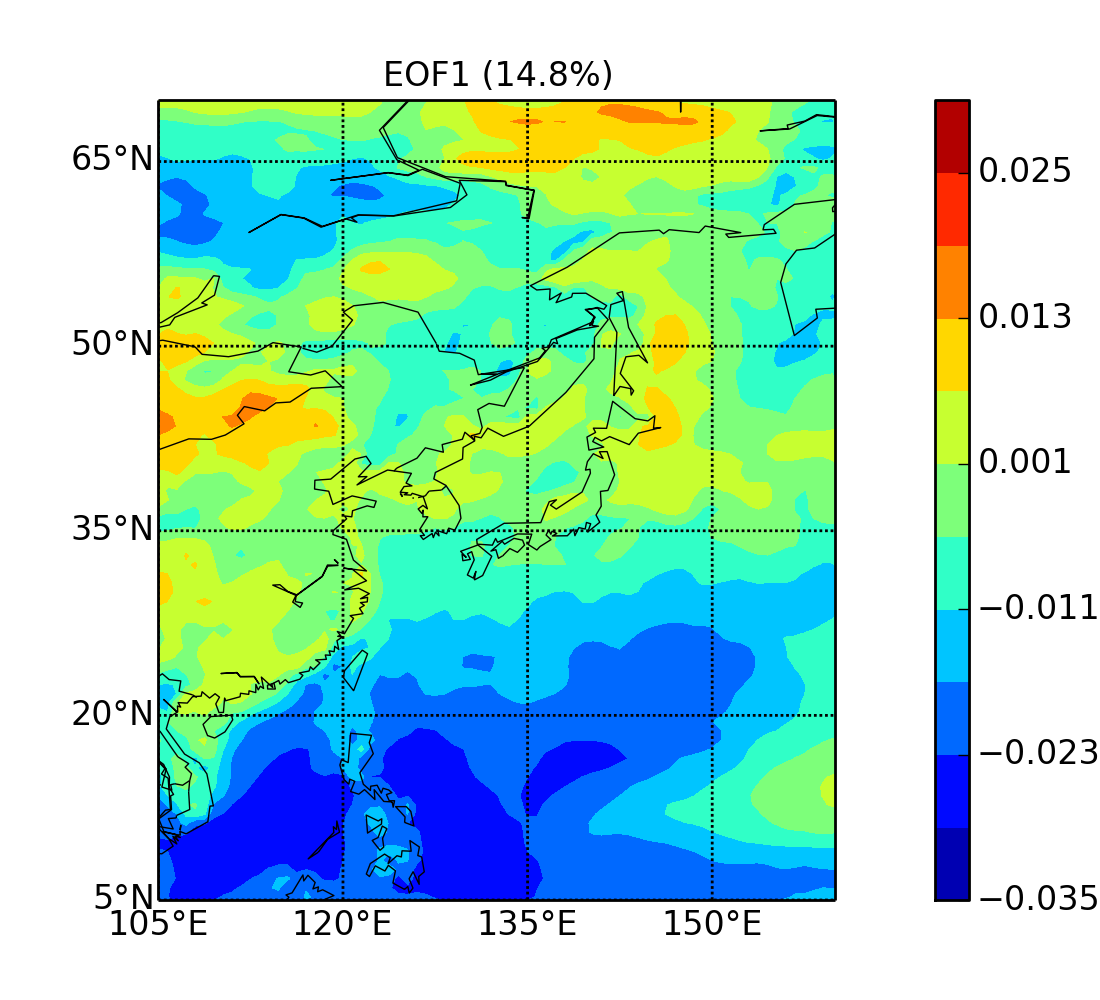
\includegraphics[width=0.5\textwidth]{eof1.png}
}\subfigure[第二模态]{\label{eof_2}
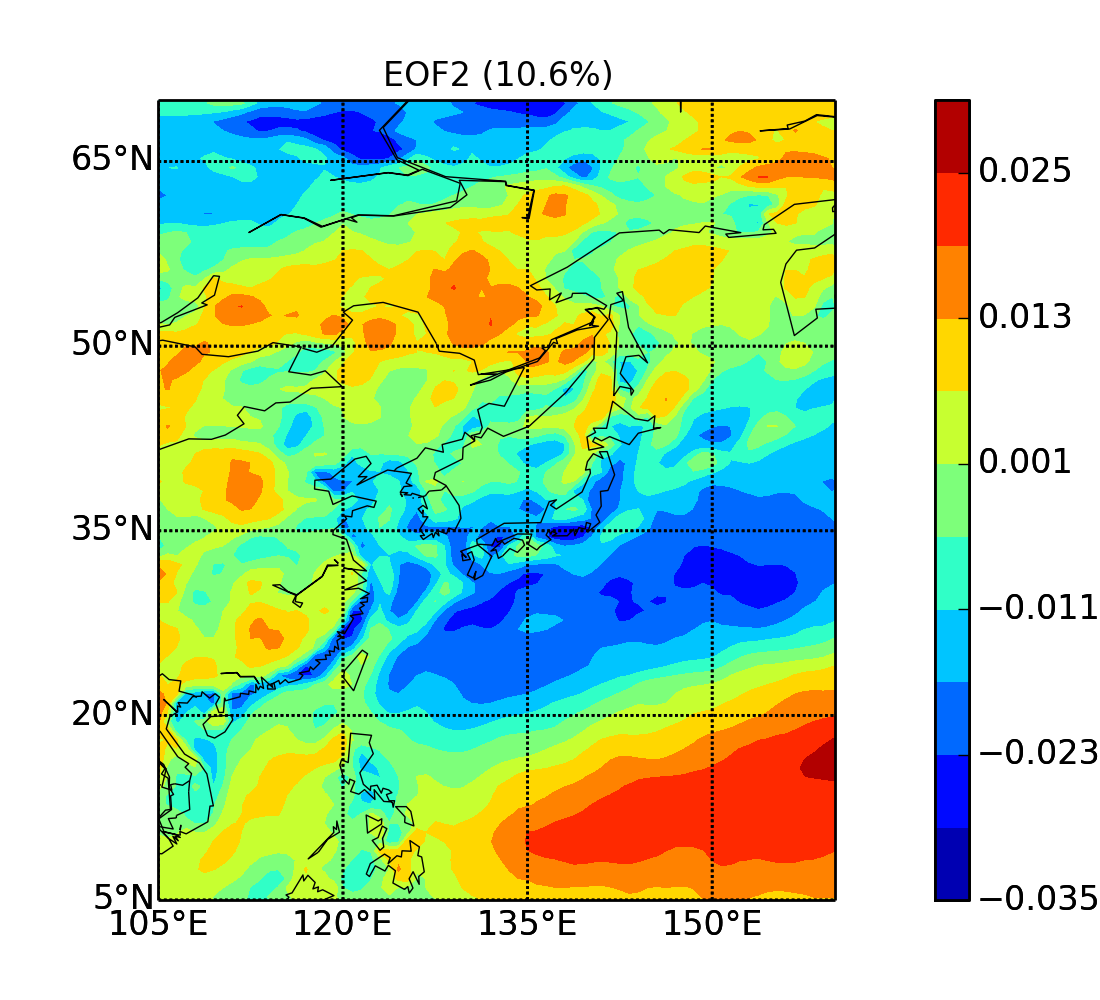
\includegraphics[width=0.5\textwidth]{eof2.png}
}
\\
\subfigure[第一模态对应的时间系数]{\label{eof_t1}
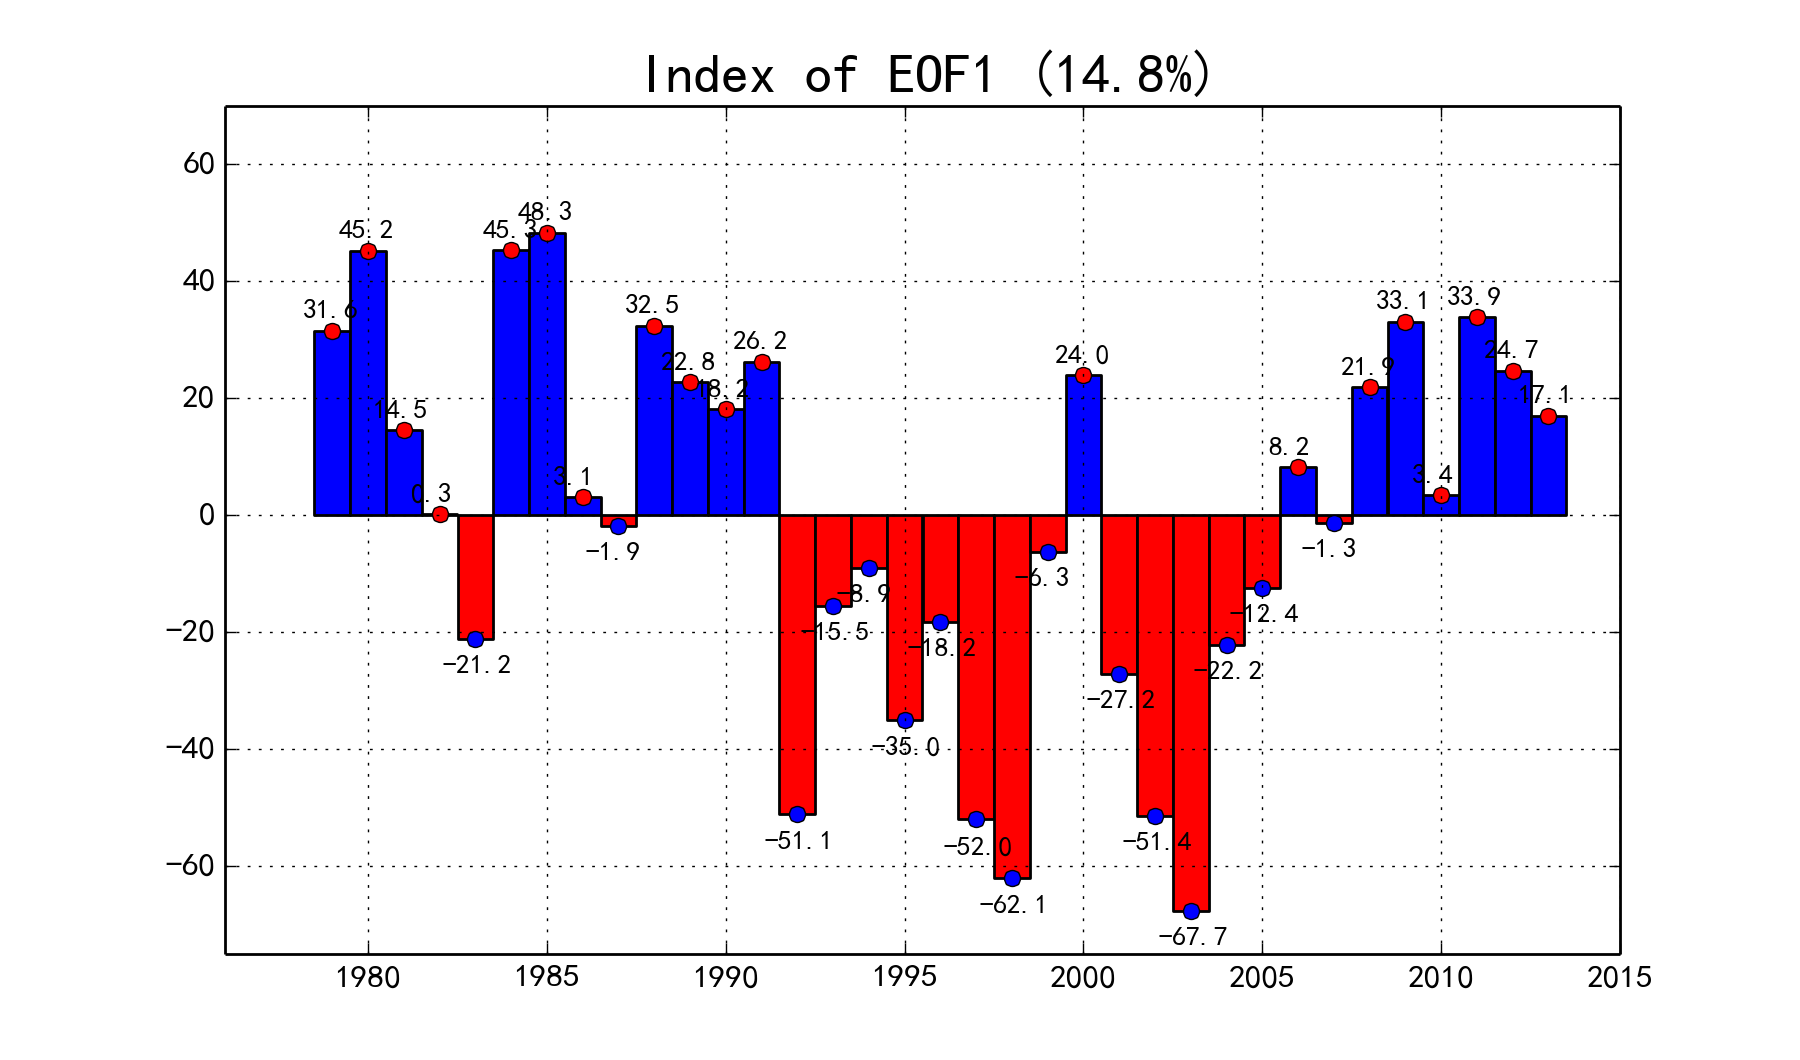
\includegraphics[width=0.5\textwidth]{t1.png}
}\subfigure[第二模态对应的时间系数]{\label{eof_t2}
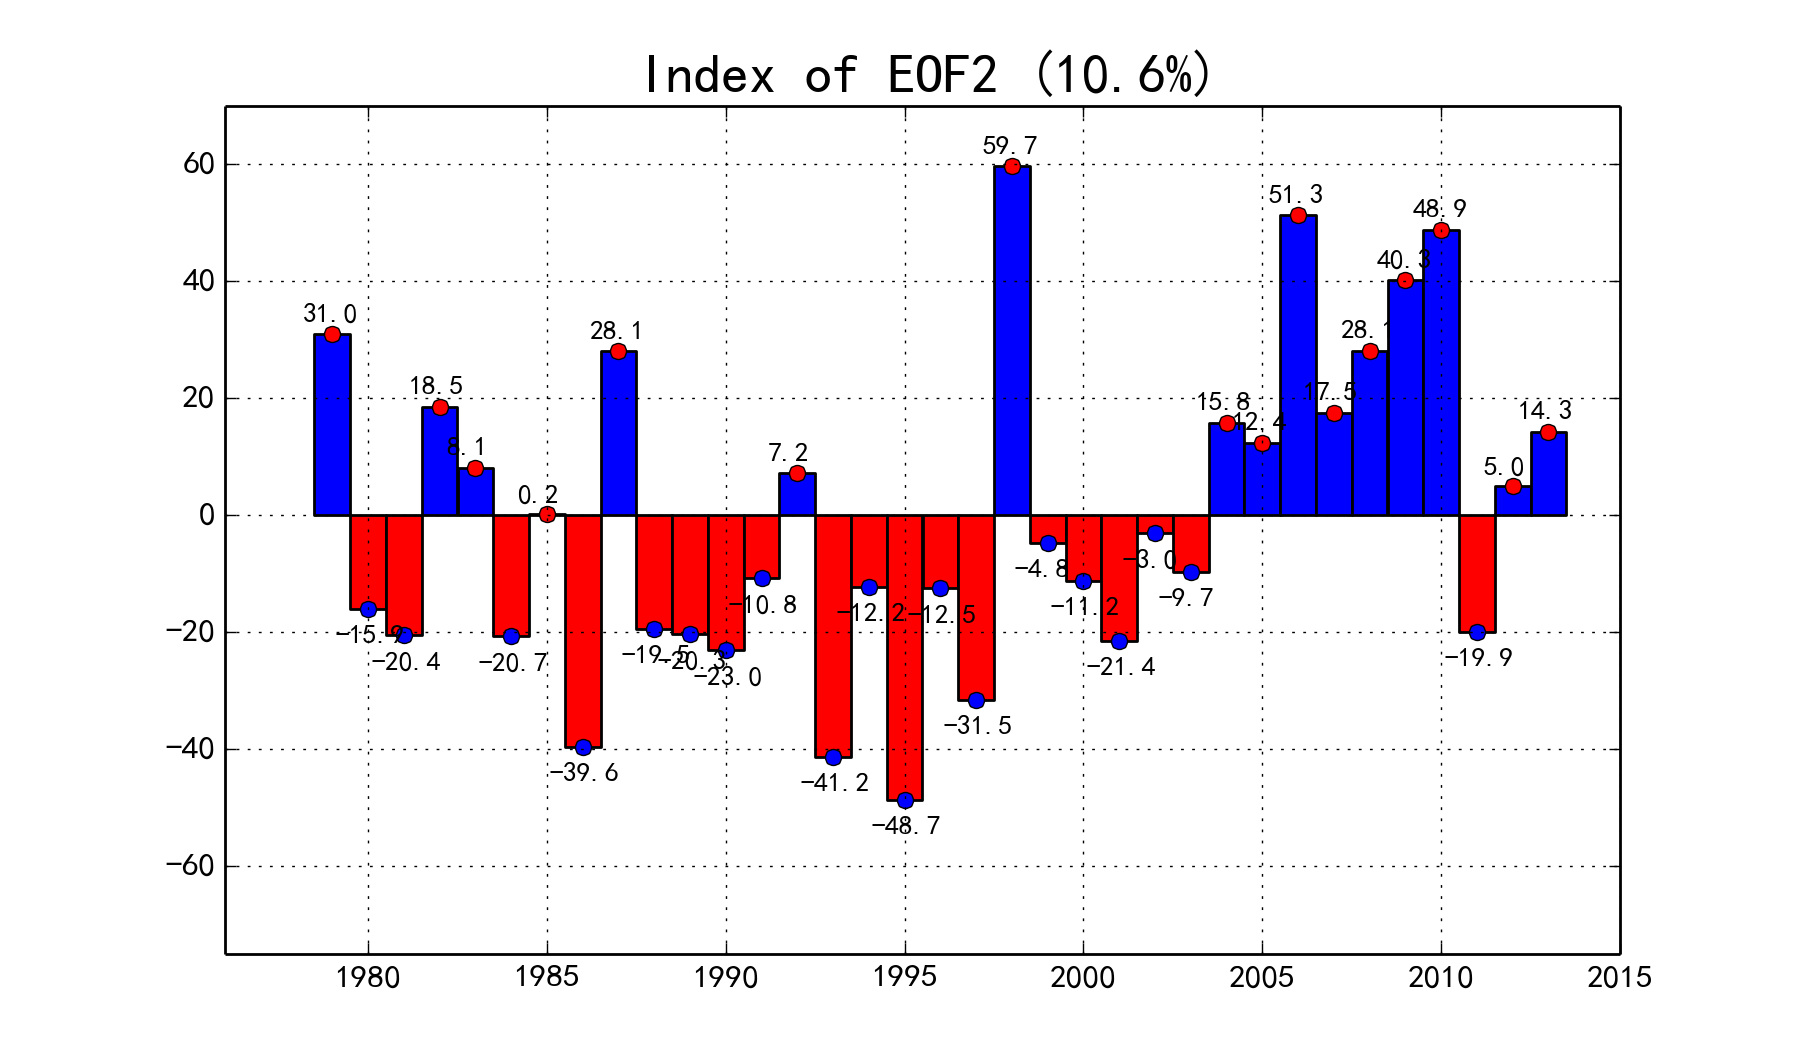
\includegraphics[width=0.5\textwidth]{t2.png}
}
\caption{ABLH的EOF分析结果(第一第二模态及其时间系数)}\label{fig:eof_12}
\end{figure}
\end{verbatim}
}


\begin{figure}[htbp]

\center
\subfigure[第一模态]{\label{eof_1}
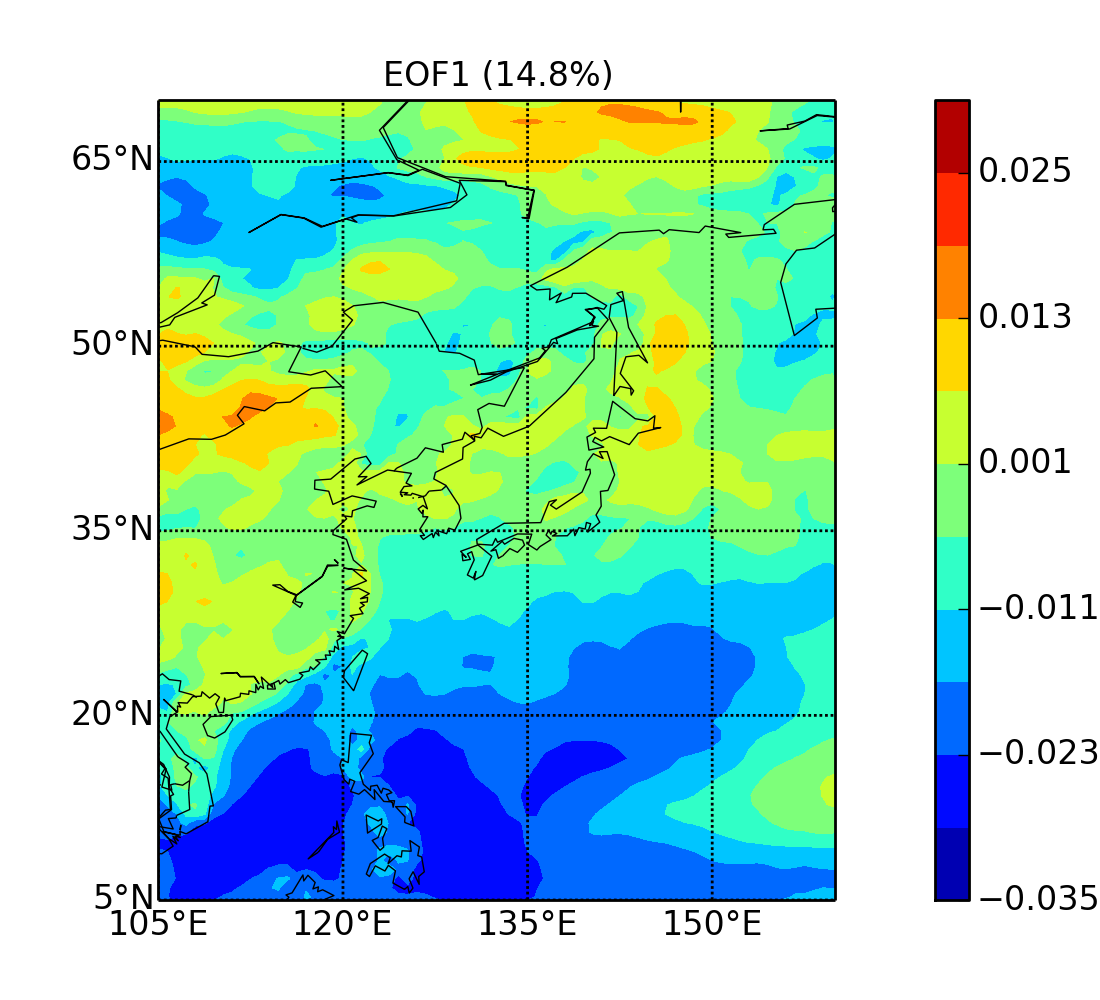
\includegraphics[width=0.5\textwidth]{eof1.png}
}\subfigure[第二模态]{\label{eof_2}
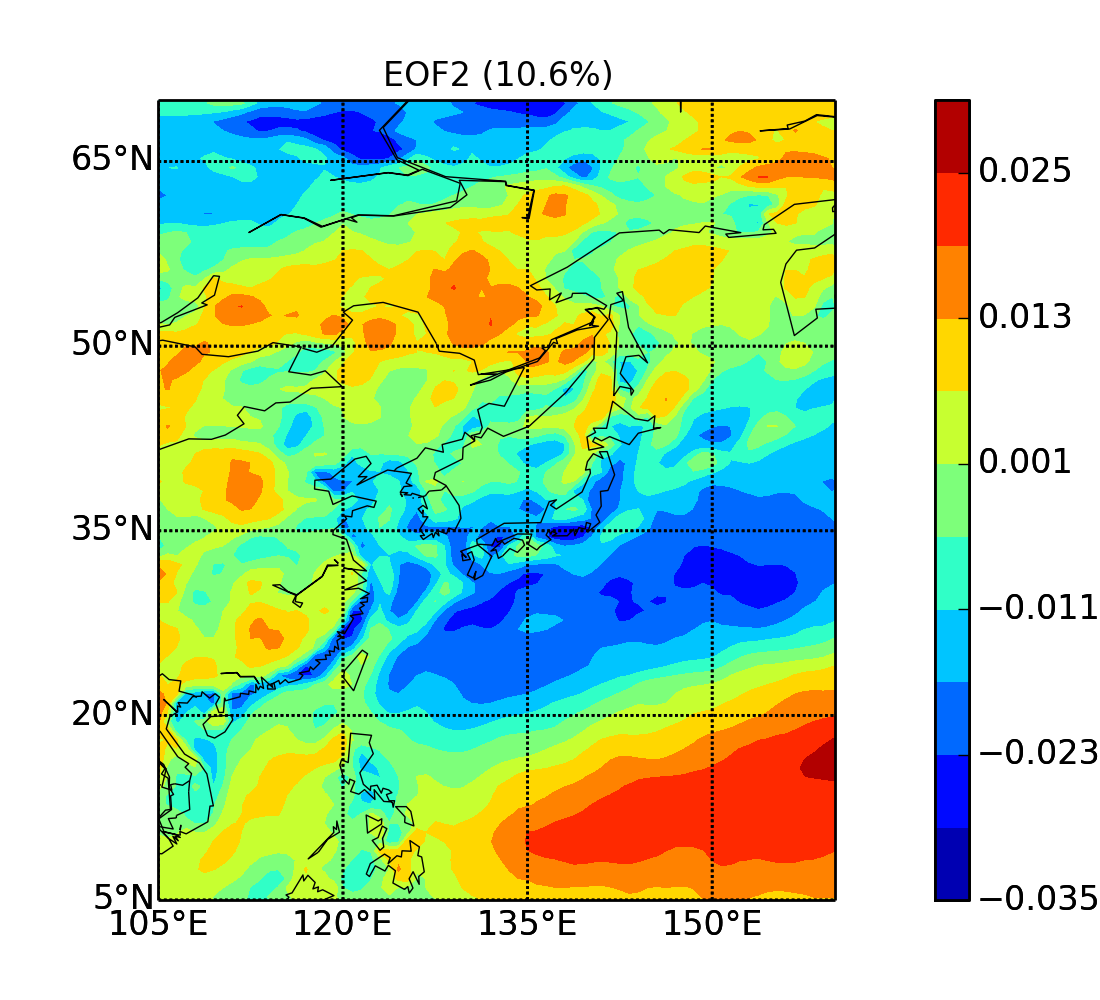
\includegraphics[width=0.5\textwidth]{eof2.png}
}
\\
\subfigure[第一模态对应的时间系数]{\label{eof_t1}
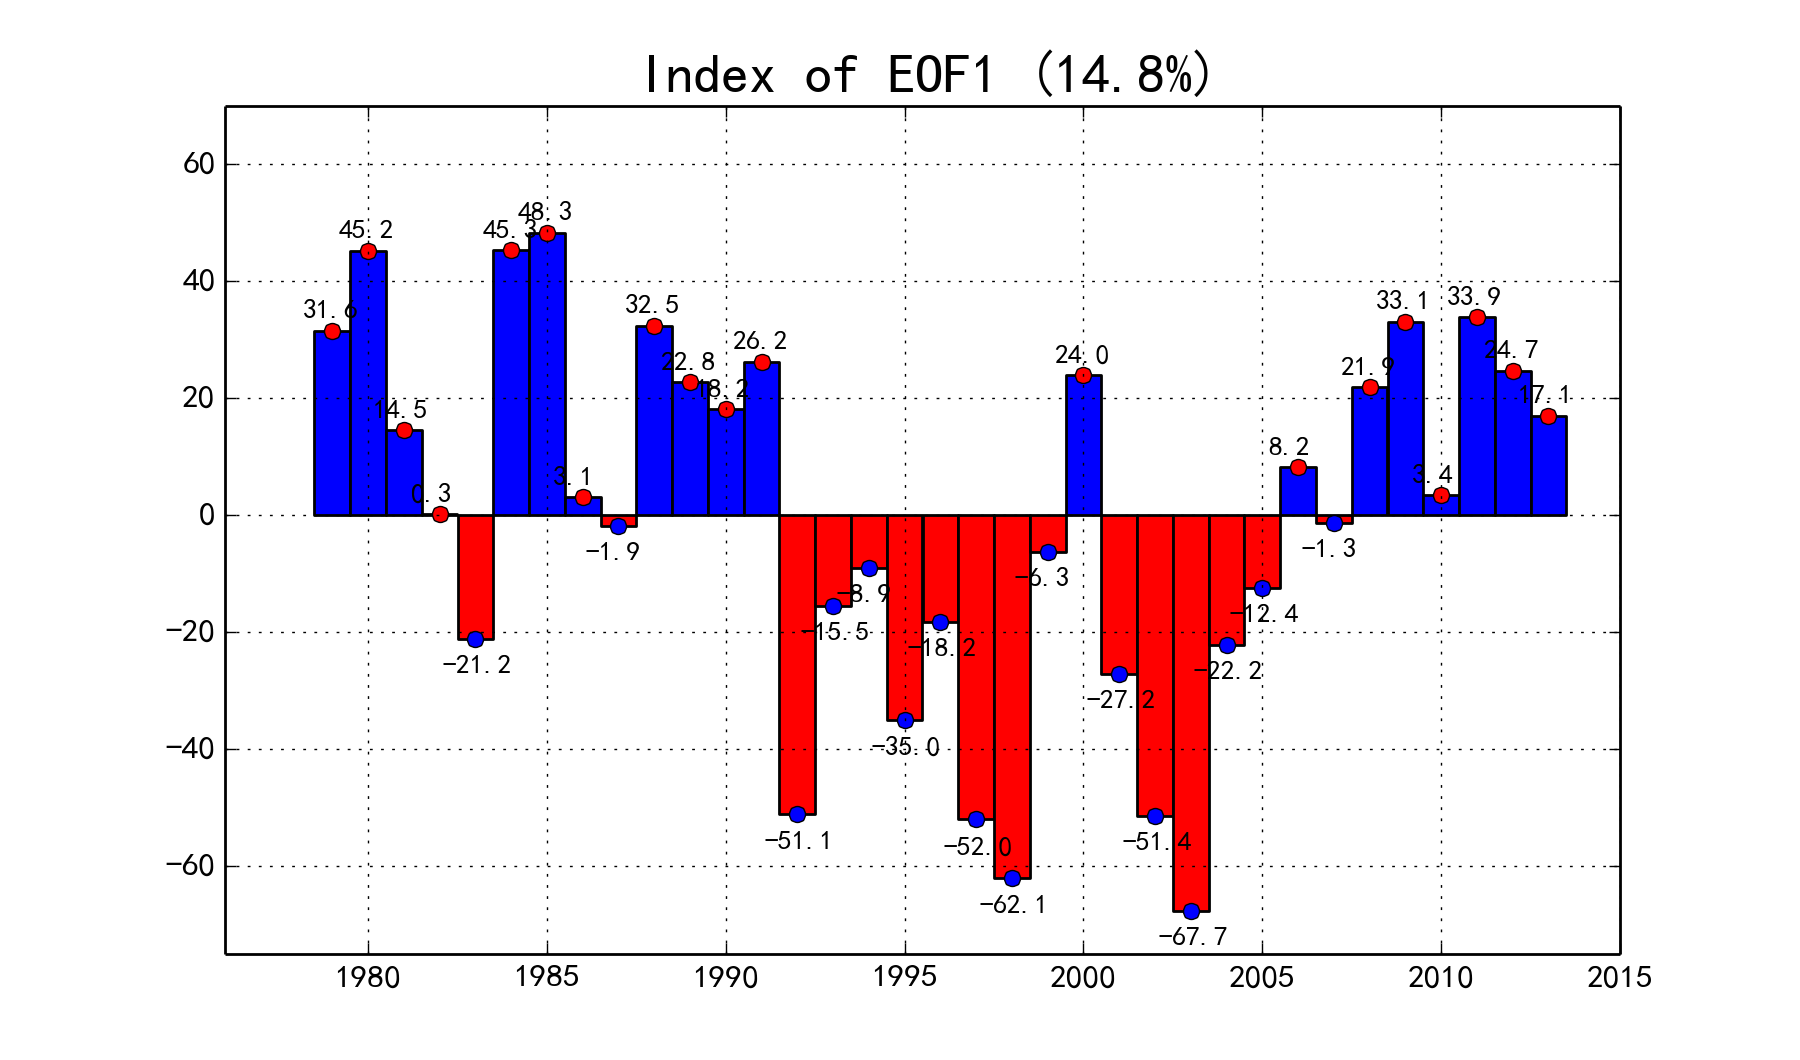
\includegraphics[width=0.5\textwidth]{t1.png}
}\subfigure[第二模态对应的时间系数]{\label{eof_t2}
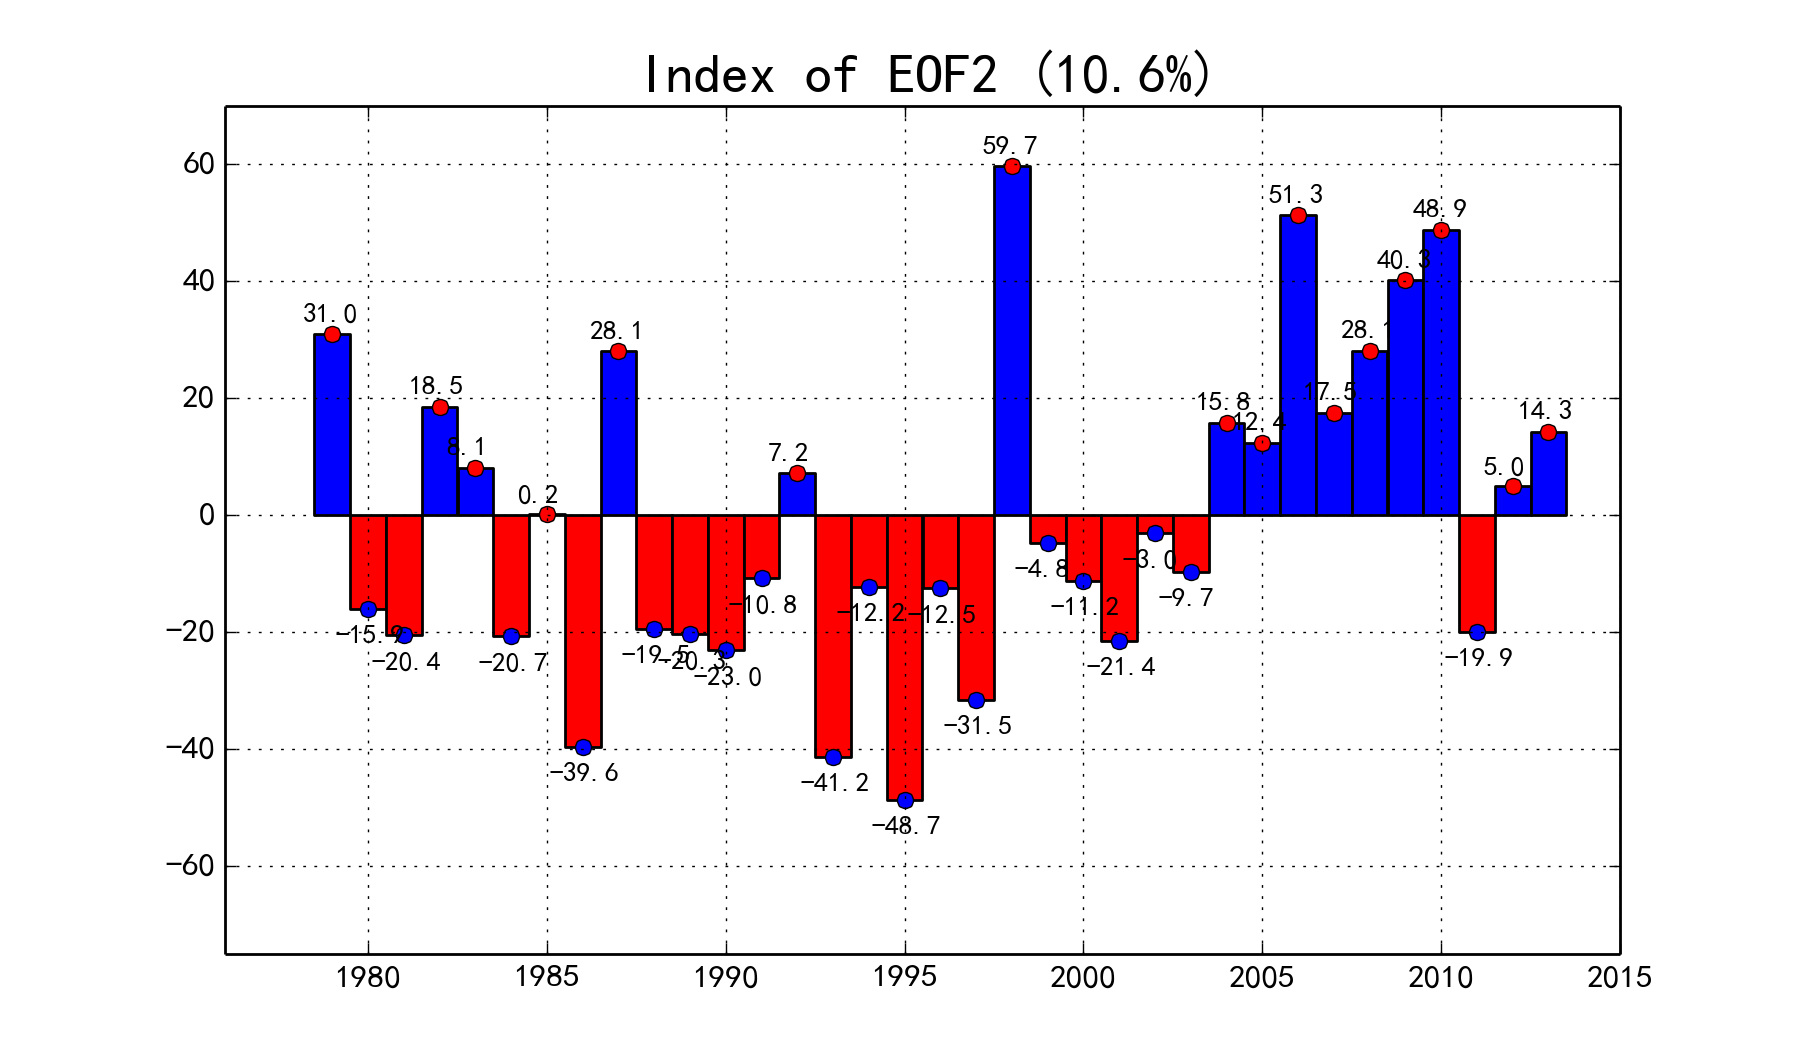
\includegraphics[width=0.5\textwidth]{t2.png}
}
\caption{ABLH的EOF分析结果(第一第二模态及其时间系数)}\label{fig:eof_12}
\end{figure}
朋友们应该也发现奥秘所在了,对,就是那个双斜线$ \backslash\backslash$的作用,双斜线在\LaTeX 排版系统中就是换行的命令,知道了这一点,大家可以随意安排自己的图片了,可以用$2\times 3$或者$3\times 2$来摆放自己插图了。


\subsection{图片文件夹的指定}
细心的朋友可能会发现生成~\ref{subfig_cn_map}~和图~\ref{cn_map}~所用的代码在指定图片路径时的写法不同,一种是全路径,另一种是只有图片名称。这是为什么呢?原因很简单。为了在写作时引用图片方便,本文在导言区写上这样的\verb|\graphicspath{{figs/color/}}|一名命令,来宏观地指定图片所存放的位置。

这一功能的好处就是,对于有的同学电子文档和打印文档所用图片色彩格式不同,这样只要一条命令就可以切换到另一个文件夹了,比较实用。
\subsection{图序号动态更新}

用word时,还有一种情况就是当我们突然想在文章中间补加一幅图时,后面图的编号及段落中对图的引用都要手工来改动,这是一件十分令人烦躁的事情,但\LaTeX 可以做到自动调整。
